\documentclass{beamer}
\usepackage[utf8]{inputenc}

\usetheme{Madrid}
\usecolortheme{default}
\usepackage{amsmath,amssymb,amsfonts,amsthm}
\usepackage{txfonts}
\usepackage{tkz-euclide}
\usepackage{listings}
\usepackage{adjustbox}
\usepackage{array}
\usepackage{tabularx}
\usepackage{gvv}
\usepackage{lmodern}
\usepackage{circuitikz}
\usepackage{tikz}
\usepackage{graphicx}

\setbeamertemplate{page number in head/foot}[totalframumber]

\usepackage{tcolorbox}
\tcbuselibrary{minted,breakable,xparse,skins}

\definecolor{bg}{gray}{0.95}
\lstset{
    language=C,
    basicstyle=\ttfamily\small,
    keywordstyle=\color{blue},
    stringstyle=\color{orange},
    commentstyle=\color{green!60!black},
    numbers=left,
    numberstyle=\tiny\color{gray},
    breaklines=true,
    showstringspaces=false,
}

%------------------------------------------------------------
\title{8.4.14}
\date{October 11,2025}
\author{EE25BTECH11011 - Navya Banavathu}
\usepackage{multicol}
\begin{document}

\frame{\titlepage}

\begin{frame}{Question}
Let $\mathbf{P}(x_1, y_1) $ and $\mathbf{Q}(x_2, y_2)$, $ y_1 < 0, y_2 < 0 $, be the endpoints of the latus rectum of the ellipse $x^2 + 4y^2 = 4$
Then, the equations of the parabolas with latus rectum $PQ$ are
\begin{enumerate}
\begin{multicols}{2}

    \item $ x^2 + 2\sqrt{3}y = 3 + \sqrt{3} $
    \item $ x^2 - 2\sqrt{3}y = 3 + \sqrt{3} $
    \item $ x^2 + 2\sqrt{3}y = 3 - \sqrt{3} $
    \item $ x^2 - 2\sqrt{3}y = 3 - \sqrt{3} $
\end{multicols}
\end{enumerate}
\end{frame}

\begin{frame}{Solution}
Consider the ellipse defined by the quadratic form
\begin{align}
\mathbf{x}^\top \mathbf{V} \mathbf{x} + 2 \mathbf{u}^\top \mathbf{x} + f = 0,
\end{align}

where
\begin{align}
\mathbf{V} = \begin{bmatrix} 1 & 0 \\ 0 & 4 \end{bmatrix}, \quad
\mathbf{u} = \mathbf{0}, \quad
f = -4.
\end{align}

The eigenvalues and eigenvectors of $\mathbf{V}$ are
\begin{align}
\lambda_1 = 1, \quad \mathbf{p}_1 = \begin{bmatrix} 1 \\ 0 \end{bmatrix}, \quad
\lambda_2 = 4, \quad \mathbf{p}_2 = \begin{bmatrix} 0 \\ 1 \end{bmatrix}.
\end{align}

The eccentricity $e$ of the ellipse is given by
\begin{align}
e = \sqrt{1 - \frac{\lambda_1}{\lambda_2}} = \sqrt{1 - \frac{1}{4}} = \frac{\sqrt{3}}{2}.
\end{align}
\end{frame}

\begin{frame}{Solution}
Define the vector
\begin{align}
\mathbf{n} = \sqrt{\lambda_2} \mathbf{p}_1 = 2 \begin{bmatrix} 1 \\ 0 \end{bmatrix} = \begin{bmatrix} 2 \\ 0 \end{bmatrix}.
\end{align}
The formula for $c$ is:
\begin{align}
c = \frac{ \mathbf{u}^\top \mathbf{n} \pm \sqrt{ e^2 (\mathbf{u}^\top \mathbf{n})^2 - \lambda_2 (e^2 - 1)( \|\mathbf{u}\|^2 - \lambda_2 f ) } }{ \lambda_2 e (e^2 - 1) }.
\end{align}

Since $\mathbf{u} = \mathbf{0}$, this simplifies to:
\begin{align}
c = \pm \frac{ \sqrt{ - \lambda_2 (e^2 - 1)( - \lambda_2 f ) } }{ \lambda_2 e (e^2 - 1) }.
\end{align}

\end{frame}

\begin{frame}{Solution}
Calculate the terms inside the square root:
\begin{align}
e^2 - 1 &= \frac{3}{4} - 1 = -\frac{1}{4}, \\
- \lambda_2 (e^2 - 1)( - \lambda_2 f ) &= -4 \times \left(-\frac{1}{4}\right) \times (-4 \times -4) = 16.
\end{align}

Thus,
\begin{align}
c &= \pm \frac{\sqrt{16}}{4 \times \frac{\sqrt{3}}{2} \times \left(-\frac{1}{4}\right)} = \mp \frac{2}{\sqrt{3}}
\end{align}


The focus $\mathbf{F}$ of the ellipse can be calculated as
\begin{align}
\mathbf{F} = \frac{c e^2 \mathbf{n}}{\lambda_2} = \frac{c \times \frac{3}{4} \times \begin{bmatrix} 2 \\ 0 \end{bmatrix}}{4} = \frac{3c}{8} \begin{bmatrix} 2 \\ 0 \end{bmatrix} = \frac{3c}{4} \begin{bmatrix} 1 \\ 0 \end{bmatrix}.
\end{align}
\end{frame}


\begin{frame}{Solution}
Choosing $c = \frac{2}{\sqrt{3}}$, we get
\begin{align}
\mathbf{F} = \frac{\sqrt{3}}{2} \begin{bmatrix} 1 \\ 0 \end{bmatrix}.
\end{align}
The endpoints $\mathbf{x}_1, \mathbf{x}_2$ of the latus rectum $PQ$, where $y_1, y_2 < 0$, satisfy the ellipse equation
\begin{align}
x^2 + 4 y^2 = 4.
\end{align}
Substituting $x = \sqrt{3}$, we find
\begin{align}
y = -\frac{1}{2},
\end{align}

so the endpoints are
\begin{align}
\mathbf{P} = \begin{bmatrix} \sqrt{3} \\ -\frac{1}{2} \end{bmatrix}, \quad
\mathbf{Q} = \begin{bmatrix} -\sqrt{3} \\ -\frac{1}{2} \end{bmatrix}
\end{align}
\end{frame}

\begin{frame}{Solution}
The midpoint (vertex) $\mathbf{V}$ of the latus rectum is
\begin{align}
\mathbf{V} = \frac{\mathbf{P} + \mathbf{Q}}{2} = \begin{bmatrix} 0 \\ -\frac{1}{2} \end{bmatrix}.
\end{align}

The length of the latus rectum is
\begin{align}
|\mathbf{P} - \mathbf{Q}| = 2 \sqrt{3} = 4a,
\end{align}

which gives
\begin{align}
a = \pm\frac{\sqrt{3}}{2}.
\end{align}


The parabola with vertex $\mathbf{V}$ and parameter $a$ has equation:
\begin{align}
x^2 = 4 a (y - y_0),
\end{align}
\end{frame}


\begin{frame}{Solution}
where $y_0 = -\frac{1}{2}$. Substituting $a =\pm\frac{\sqrt{3}}{2}$, we get


\textbf{Case 1:} $a = +\dfrac{\sqrt{3}}{2}$\\
\begin{align}
x^2 - 2\sqrt{3}y &= 3 + \sqrt{3}.
\end{align}

\textbf{Case 2:} $a = -\dfrac{\sqrt{3}}{2}$\\
\begin{align}
x^2 + 2\sqrt{3}y &= 3 - \sqrt{3}.
\end{align}

Hence, the equations of the required parabolas are
\begin{align}
\boxed{
x^2 - 2\sqrt{3}y = 3 + \sqrt{3}
\quad \text{and} \quad
x^2 + 2\sqrt{3}y = 3 - \sqrt{3}.
}
\end{align}
\end{frame}

\begin{frame}[fragile]{ Code (C)}
\begin{block}{Part 1}
\begin{lstlisting}[language=C, basicstyle=\ttfamily\small, keywordstyle=\color{blue}, frame=single]
#include <stdio.h>
#include <math.h>

int main() {
    // Ellipse: x^2 + 4y^2 = 4
    // Latus rectum endpoints y < 0
    double x1 = sqrt(3.0);
    double x2 = -sqrt(3.0);
    double y1 = -0.5;
    double y2 = -0.5;

    // Midpoint (vertex of parabola)
    double vx = (x1 + x2) / 2.0;
    double vy = (y1 + y2) / 2.0;
\end{lstlisting}
\end{block}
\end{frame}




\begin{frame}[fragile]{ Code (C)}
\begin{block}{Part 2}
\begin{lstlisting}[language=C, basicstyle=\ttfamily\small, keywordstyle=\color{blue}, frame=single]
    // Length of latus rectum
    double L = x1 - x2; 
    double a = L / 4.0; 

    // Case 1: a positive
    double f1 = -4 * a * vy; // move vy to RHS
    printf("Equation of parabola 1:\n");
    printf("x^2 - %.3lf*y = %.3lf\n", 4*a, f1);

    // Case 2: a negative
    a = -a;
    double f2 = -4 * a * vy;
    printf("Equation of parabola 2:\n");
    printf("x^2 - %.3lf*y = %.3lf\n", 4*a, f2);

    return 0;
}
\end{lstlisting}
\end{block}
\end{frame}

\begin{frame}[fragile]{Python Code}
\begin{block}{Part 1}
\begin{lstlisting}[language=Python, basicstyle=\ttfamily\small, keywordstyle=\color{blue}, frame=single]
import ctypes
import numpy as np
import matplotlib.pyplot as plt

libm = ctypes.CDLL('code14.dll')
libm.sqrt.argtypes = [ctypes.c_double]
libm.sqrt.restype = ctypes.c_double

def c_sqrt(x):
    return libm.sqrt(x)

# Ellipse parameters
a_ellipse = 2.0
b_ellipse = 1.0

e = c_sqrt(1 - (b_ellipse**2) / (a_ellipse**2))
\end{lstlisting}
\end{block}
\end{frame}


\begin{frame}[fragile]{Python Code}
\begin{block}{Part 2}
\begin{lstlisting}[language=Python, basicstyle=\ttfamily\small, keywordstyle=\color{blue}, frame=single]
c = a_ellipse * e
# Latus rectum endpoints (y < 0)
xP, yP = c, -0.5
xQ, yQ = -c, -0.5

xV = (xP + xQ) / 2
yV = (yP + yQ) / 2

lengthPQ = np.sqrt((xP - xQ)**2 + (yP - yQ)**2)
a_p = lengthPQ / 4
# Parabola coefficient 2 * sqrt(3)
coeff = 2 * np.sqrt(3)

# Constant in parabola equation x^2 - 2√3 y = constant
constant = -coeff * yV
print(f"Parabola equation: x^2 - 2√3 y = {constant:.4f}")
\end{lstlisting}
\end{block}
\end{frame}

\begin{frame}[fragile]{Python Code: Plotting}
\begin{block}{Part 3}
\begin{lstlisting}[language=Python, basicstyle=\ttfamily\small, keywordstyle=\color{blue}, frame=single]
theta = np.linspace(0, 2*np.pi, 400)
x_ellipse = a_ellipse * np.cos(theta)
y_ellipse = b_ellipse * np.sin(theta)

# Parabola: x^2 = 2√3 (y + 0.5)
# => y = (x^2) / (2√3) - 0.5
x_parabola = np.linspace(-4, 4, 400)
y_parabola = (x_parabola**2) / (2 * np.sqrt(3)) - 0.5

plt.figure(figsize=(8, 6))
plt.plot(x_ellipse, y_ellipse, label='Ellipse: $x^2 + 4y^2 = 4$', color='blue')
plt.plot(x_parabola, y_parabola, label='Parabola', color='red')
# Mark latus rectum endpoints and vertex
plt.scatter([xP, xQ], [yP, yQ], color='green', label='Latus Rectum Endpoints P, Q')
plt.scatter(xV, yV, color='purple', label='Vertex V')
\end{lstlisting}
\end{block}
\end{frame}

\begin{frame}[fragile]{Python Code: Plotting}
\begin{block}{Part 4}
\begin{lstlisting}[language=Python, basicstyle=\ttfamily\small, keywordstyle=\color{blue}, frame=single]
plt.axhline(0, color='black', linewidth=0.5)
plt.axvline(0, color='black', linewidth=0.5)

plt.title('Ellipse and Parabola with Latus Rectum')
plt.xlabel('x')
plt.ylabel('y')
plt.legend()
plt.grid(True)
plt.axis('equal')

# Save the plot
plt.savefig('fig14.png', dpi=300)
plt.show()
\end{lstlisting}
\end{block}
\end{frame}

\begin{frame}{Graphical Representation}
    \begin{figure}
        \centering
        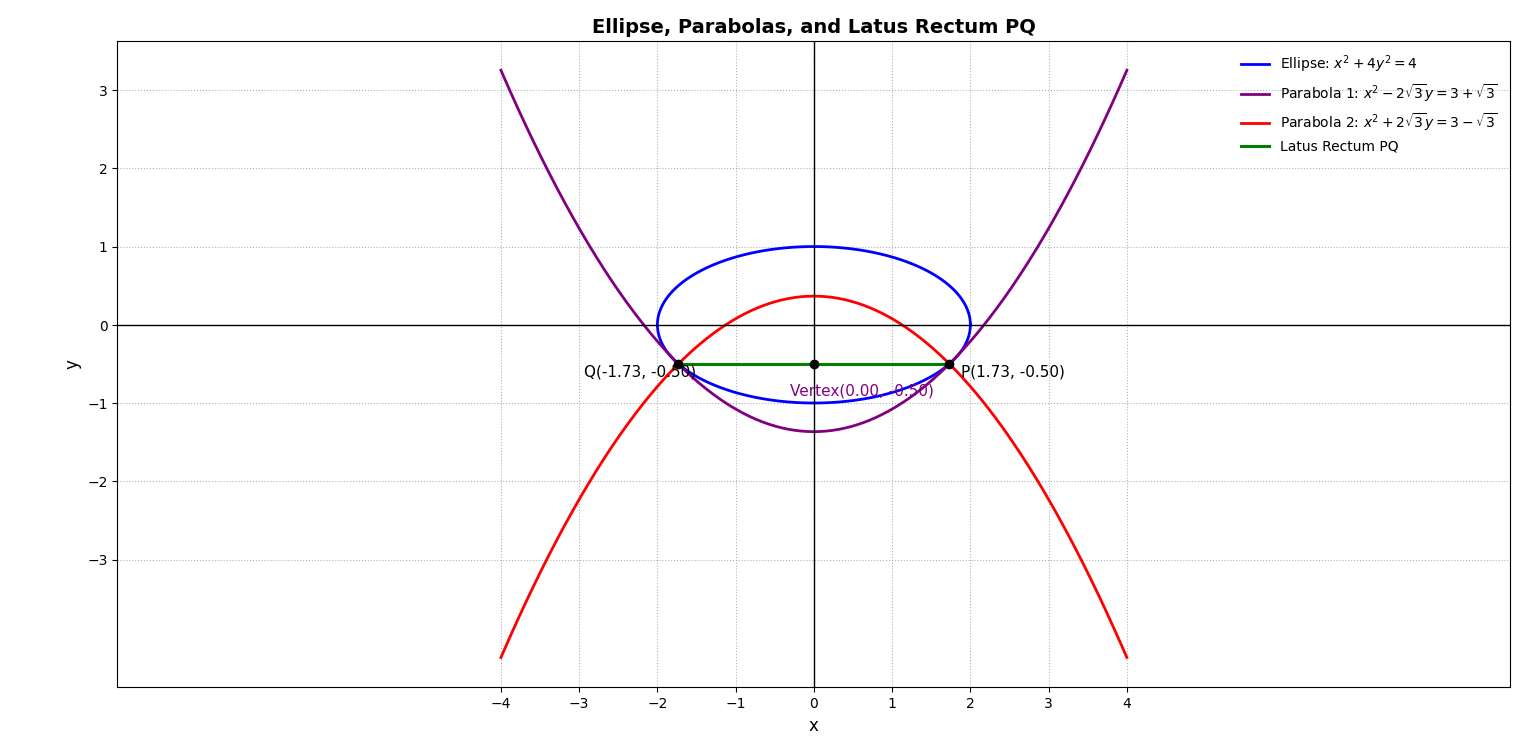
\includegraphics[width=0.8\columnwidth]{../beamer/figs/fig14.png}
    \end{figure}
\end{frame}

\end{document}

